% 同轴叠画采用教材式不同高度的区间括线；本文件会嵌入各份TeX。
\definecolor{SetBlue}{RGB}{66,132,177}
\newcommand{\SetBaseAxis}{%
  \draw[->,line width=0.55pt] (-0.7,0)--(11.2,0) node[right] {$x$};
  \foreach \t in {0,2,3,7,10}{\draw[line width=0.45pt] (\t,0)--(\t,0.065);\node[below=3pt,font=\small] at (\t,0) {$\t$};}}
\newcommand{\SetBlankAxes}{%
  \begin{center}\begin{tikzpicture}[x=0.92cm,y=1cm,font=\small]
  \path (-0.7,0) rectangle (11.2,1.25);\SetBaseAxis
  \end{tikzpicture}\end{center}}
\newcommand{\SetNumberLines}{%
  \begin{center}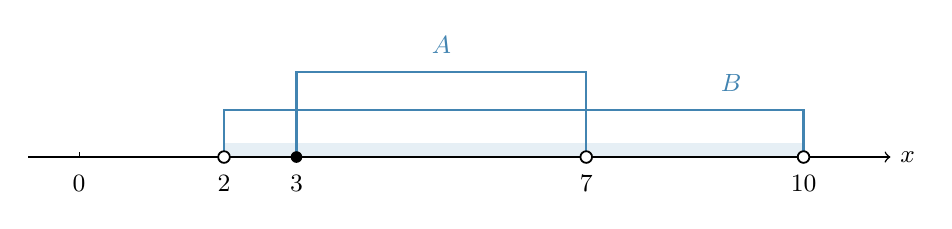
\begin{tikzpicture}[x=0.92cm,y=1cm,font=\small]
  \fill[SetBlue!13] (2,0) rectangle (10,0.18);
  \SetBaseAxis
  \draw[SetBlue,line width=0.8pt] (3,0)--(3,1.08)--(7,1.08)--(7,0);
  \draw[SetBlue,line width=0.8pt] (2,0)--(2,0.60)--(10,0.60)--(10,0);
  \node[SetBlue,above=3pt] at (5,1.08) {$A$};
  \node[SetBlue,above=3pt] at (9,0.60) {$B$};
  \foreach \t in {2,7,10}{\filldraw[fill=white,draw=black,line width=0.65pt] (\t,0) circle (2.1pt);}
  \fill (3,0) circle (2.1pt);
  \end{tikzpicture}\end{center}}
\newcommand{\QuadraticCases}{%
  \begin{center}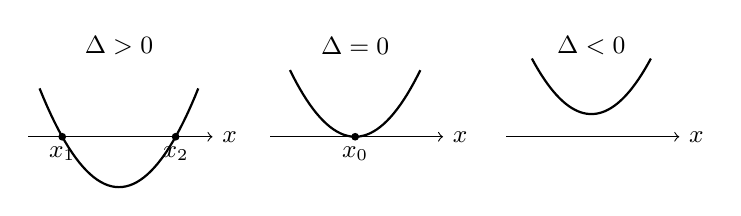
\begin{tikzpicture}[x=0.72cm,y=0.64cm,font=\small]
  \begin{scope}\draw[->] (-1.6,0)--(1.65,0) node[right] {$x$};\draw[thick,domain=-1.4:1.4,samples=45] plot (\x,{\x*\x-1});\fill (-1,0) circle (1.4pt);\fill (1,0) circle (1.4pt);\node[below] at(-1,0){$x_1$};\node[below] at(1,0){$x_2$};\node at(0,1.8){$\Delta>0$};\end{scope}
  \begin{scope}[xshift=3cm]\draw[->] (-1.5,0)--(1.55,0) node[right] {$x$};\draw[thick,domain=-1.15:1.15,samples=40] plot (\x,{\x*\x});\fill (0,0) circle (1.4pt);\node[below] at(0,0){$x_0$};\node at(0,1.8){$\Delta=0$};\end{scope}
  \begin{scope}[xshift=6cm]\draw[->] (-1.5,0)--(1.55,0) node[right] {$x$};\draw[thick,domain=-1.05:1.05,samples=40] plot (\x,{\x*\x+0.45});\node at(0,1.8){$\Delta<0$};\end{scope}
  \end{tikzpicture}\end{center}}
